\section{Pattern Matching der \acs{fhir}-Profile mit den Konfigurationsvariablen} \label{sec:pattmach}

Nach der Erkennung der 701 relevanten Konfigurationsvariablen und der Datendefinition, wurde das Pattern Matching durchgeführt, um bestimmte Muster zwischen Parametern der \ac{fhir}-Profile und Attributen der \ac{copra}-Konfigurationsvariablen zu erkennen. 

Der erste Schritt für das Pattern Matching war die Zuordnung der \ac{fhir}-Profile mit den Konfigurationsvariablen durch eine unscharfe Suche. Für diesen Zweck wurden der Parameter \texttt{profile\_name} der Tabelle \texttt{mii\_icu} zusammen den Parametern \texttt{name} und \texttt{description} der Tabelle \texttt{co6\_config \_variables} in einem \ac{csv}-Datei extrahiert. 

Mit einem Python-Skript und der extrahierten \ac{csv}-Datei wurde die unscharfe Suche durchgeführt. Dieser Prozess liefert einen Datensatz mit 400 Paaren von zugeordneten Profilen mit Konfigurationsvariablen. 355 Paaren davon waren falsche Zuordnungen, wie die Beispiele der \ref{tab:wrongpaar} zeigen.

\begin{lstlisting}[language=python, caption={[Python-Skript für das Pattern Matching] Python-Skript für das Pattern Matching. Die Option \glqq token\_set\_ratio\grqq{} ermöglicht eine flexiblere fuzzy-Suche (\ref{sub:levdist}), denn die Länge der Namen der Profile, Namen und  Beschreibungen der Konfigurationsvariablen deutlich unterschiedlich sind.} , captionpos=b, label=list:testr]
from thefuzz import process, fuzz  # Bibliotheken laden

with open("profils_names.csv") as fp: # Datei mit den Namen der Profile
prn = fp.readlines() # Name der Profile
prn = [x.strip() for x in prn] 

with open("config_vars_names.csv") as fc: # Datei mit den Konfigurationsvariablen
cvn = fc.readlines() # Konfigurationsvariablen
cvn = [x.strip() for x in cvn]

for profil in prn: # Bei jeden Namen der Profile
  match_ratios = process.extract(profil, cvn, scorer=fuzz.token_set_ratio) # Liste der passenden Konfigurationsvariablen.
  for prn_match_cvn in match_ratios: 
    print(profil, prn_match_cvn) # Liste der Paaren "Profile - Konfigurationsvariablen"
   
\end{lstlisting}

\begin{table}[ht]
	\centering 
	\caption[Beispiele von falsch zugeordneten \acs{fhir}-Profile]{Beispiele von falsch zugeordneten \acs{fhir}-Profile. Die Namen der Konfigurationsvariablen und deren Beschreibung sind durch \glqq-\grqq{} getrennt.}
	\label{tab:wrongpaar}
	\begin{tabular}{|l|l|}
		\hline
		\bfseries Profil & \bfseries Konfigurationsvariable \\ \hline
		Arterieller Druck & ICP - Intrakranialer Druck \\ \hline
		Atemfrequenz & HF - Herzfrequenz \\ \hline
        Rechtsatrialer Druck & CPP - Zerebraler Perfusionsdruck \\ \hline
        Venoeser Druck & PAP - Pulmunalarterieller Druck \\ \hline
	\end{tabular}
\end{table}

Nach dem vorherigen Ergebnis der unscharfen Suche wurden die \ac{fhir}-Profile und die Konfigurationsvariablen nochmal analysiert. Dieses Mal mit \ac{sql}-Abfragen mit \acp{regex} in den WHERE-Bedingungen. Für dieses Verfahren wurden Informationen der Spalten \texttt{profile\_name} und \texttt{loinc} der Tabelle \texttt{mii\_icu} benutzt, um Muster in den Spalten \texttt{name} und \texttt{description} der Tabelle \texttt{co6\_config\_variables} zu identifizieren. Die \ref{fig:mapping} zeigt eine Darstellung der angewandten Parameter der Tabellen und deren Zusammenführung in dem Pattern Matching-Prozess.

\clearpage

\begin{figure}[ht]
	\centering
	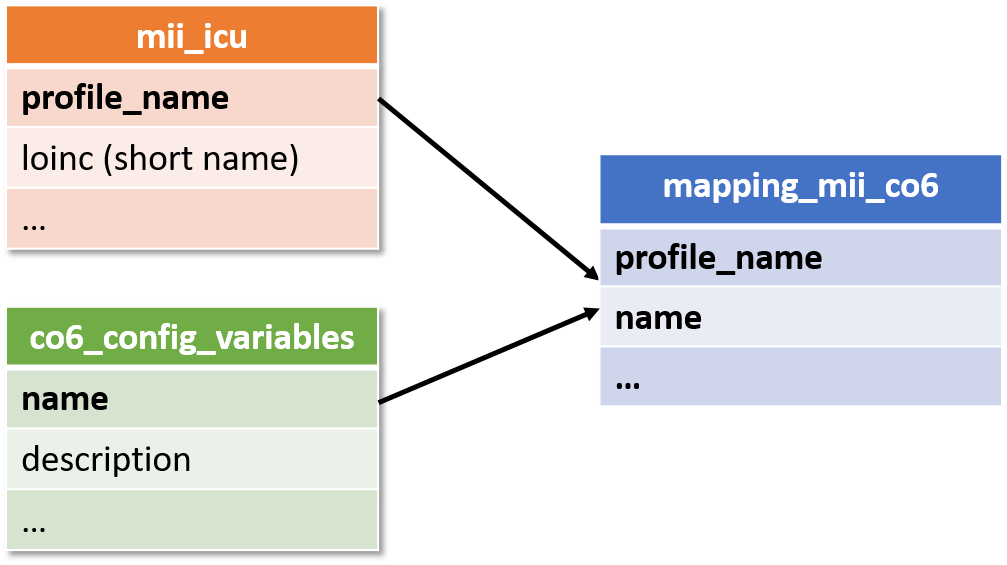
\includegraphics[height=5.5cm]{figures/mapping}
	\caption[Zuordnung der Konfigurationsvariablen mit den \acs{fhir}-Profilen]{Schematische Darstellung der Zuordnung der Spalte \texttt{profile\_name} und die Short Names der \acs{loinc}-Codes in der Spalte \texttt{loinc} der Tabelle \texttt{mii\_icu} mit den Spalten \texttt{name} und \texttt{description} der Tabelle \texttt{co6\_config\_variables}. Das Ergebnis der Zuordnung wird in der Tabelle \texttt{mapping\_mii\_co6} gespeichert.}
	\label{fig:mapping}
\end{figure}

Wichtig für die Definition der \acs{regex} bei der Anwendung dieses Verfahrens ist die Auswahl von Teilwörtern (\ref{subsec:pattmatch}) oder Kombinationen davon, die die \ac{fhir}-Profile charakterisieren. Denn diese Teilwörter sind in den meisten Fällen Fachtermini oder Teile von Fachbegriffen und können wieder in den Namen oder Beschreibungen der Konfigurationsvariablen gefunden werden.

 Manche Teilwörter in den Profilnamen sind sehr allgemein und befinden sich in mehreren Profilen und auch in zahlreichen Namen und Beschreibungen der Konfigurationsvariablen, z. B. \glqq druck\grqq{}. Das hat zufolge, dass viele Konfigurationsvariablen falsch einem Profil durch die Nutzung von nur einem von diesen Teilwörtern zugeordnet werden könnten. Solche Teilwörter wurden in Kombination mit anderen benutzt, um das Pattern Matching zu verfeinern und die Trefferquote zu erhöhen. Hier ist auch die Menge und Länge der angewandten Teilwörter entscheidend, denn die Anwendung von vielen oder zu langen Teilwörtern liefert auch kein Ergebnis. Aus diesem Grund wurde bei der Schreibung der \ac{sql}-Abfragen je \ac{fhir}-Profil solange die Definition der \ac{regex} getestet, bis die optimale Menge und Länge der Teilwörter in der \ac{regex} gefunden wurde, die die genaue Menge an Konfigurationsvariablen geliefert hatten.

Der Code \ref{list:pattdruck} zeigt beispielhaft die \ac{sql}-Abfrage mit \ac{regex} für die gleichzeitige Erkennung mehrerer allgemeiner Teilwörter des Profils \glqq Mittlerer Beatmungsdruck\grqq{} in der Tabelle der Konfigurationsvariablen, um \ac{fhir}-Profile und Konfigurationsvariablen zu zuordnen.
\clearpage
\begin{lstlisting}[language=SQL, caption={[SQL-Abfrage mit allgemeinen Teilwörtern] SQL-Abfrage mit allgemeinen Teilwörtern.} , captionpos=b, label=list:pattdruck]
select 
  name, 
  description, 
  id, 
  unit
from mii_copra.co6_config_variables 
where name ~* 'mitt.+atm.+druc'
or description ~* 'mitt.+atm.+druc'
or name ~* 'mea.+pres.+(resp|vent)'
or description ~* 'mea.+pres.+(resp|vent)'
;
\end{lstlisting}

In dem Code \ref{list:pattdruck} werden die Spalten \texttt{name} und \texttt{description} der Tabelle \texttt{co6\_config\_variables} gleichzeitig zur Erkennung von Mustern untersucht. In der definierten \ac{regex} dieser \ac{sql}-Abfrage wird die Tilde \glqq$\sim$\grqq{} gefolgt von einem Sternchen \glqq$\ast$\grqq{} benutzt, um Groß- und Kleinschreibung nicht zu berücksichtigen. Die Teilwörter \glqq mitt\grqq{}, \glqq atm\grqq{} und \glqq druc\grqq{} des Profils \glqq Mittlerer Beatmungsdruck\grqq{} verbunden durch \glqq .+\grqq{}, für eine Folge von beliebigen Zeichen, haben das Ergebnis der \ref{tab:mittatmdruck} geliefert. Die Teilwörter \glqq mea\grqq{}, \glqq pres\grqq{} und die Gruppierung mit den Alternativen \glqq resp\grqq{} oder \glqq vent \grqq{} wurden benutzt, um den Name (Mean pressure Respiratory system airway --on ventilator) auf Englisch und den \glqq Short Name\grqq{} (Mean Pres on vent Airway) zu berücksichtigen.

\begin{longtable}{|l|p{5cm}|}
	\caption[Erkannte Konfigurationsvariablen durch eine \acs{regex} mit einer Kombination von allgemeinen Teilwörtern]{Erkannte Konfigurationsvariablen bei der Anwendung der Kombination von allgemeinen Teilwörtern. Das \ac{fhir}-Profil Mittlerer Beatmungsdruck wurde drei Konfigurationsvariablen zugeordnet.}
	\label{tab:mittatmdruck}
	\endfirsthead
		\hline
		\bfseries \texttt{name} & \bfseries \texttt{description} \\ \hline
		  Beatmung\_MS\_VisionA\_MAP & gemessener Mittlerer Atemwegsdruck unter HFO bei Alpha Vision \\ \hline
		  Beatmung\_ES\_VisionA\_MAP & Mittlerer Atemwegsdruck (MAP) \\ \hline                             
		  Beatmung\_MS\_Servoi\_Pmean & Mittlerer Atemwegsdruck \\ \hline   
\end{longtable}

Andere Teilwörter wie \glqq intrakraniell\grqq{} können hingegen alleine benutzt oder zerteilt werden, ohne die Trefferquote des Pattern Matchings zu reduzieren, weil sie nicht sehr häufig in den \ac{fhir}-Profilnamen und in den Namen und Beschreibungen der Konfigurationsvariablen vorkommen, sodass durch diese Teilwörter die \ac{fhir}-Profile besser charakterisiert werden. Der Code \ref{list:pattermatc} zeigt beispielhaft die \ac{sql}-Abfrage mit der Definition der \ac{regex} mit nur einem Teilwort, um die passenden Konfigurationsvariablen zu dem \ac{fhir}-Profil \glqq Intrakranieller Druck\grqq{} zu detektieren.

\begin{lstlisting}[language=SQL, caption={[SQL-Abfrage mit einem seltenen Teilwort] SQL-Abfrage mit einem seltenen Teilwort.}, captionpos=b, label=list:pattermatc]
select 
  name, 
  description, 
  id, 
  unit
from mii_copra.co6_config_variables 
where name ~* 'intra[ck]'
or description ~* 'intra[ck]'
;
\end{lstlisting}

In dem Code \ref{list:pattermatc} werden, wie bei dem Code \ref{list:pattdruck}, die Spalten \texttt{name} und \texttt{description} gleichzeitig untersucht. In diesem Beispiel befinden sich in den eckigen Klammern die Buchstaben \glqq c\grqq{} und \glqq k\grqq{}, um die Teilwörter \glqq intrakraniell\grqq{} oder \glqq intracranial\grqq{}, auf Englisch, zu identifizieren.

Ein vorher genannter Aspekt ist die allgemeine, umgangssprachliche Anwendung der \ac{loinc}-\glqq Short Names\grqq{} vom Personal des Gesundheitswesens und wie dieser Parameter in der Konfigurationsvariablen zu finden ist. Ein Beispiel des Ergebnisses eines Pattern Matchings, um \glqq Short Names\grqq{} der \ac{loinc}-Codes zu berücksichtigen ist in der \ref{tab:shortnamepattern} dargestellt. In diesem Beispiel ist die Erkennung eines \glqq Short Name\grqq{} in der Spalte \texttt{name} der Tabelle \texttt{co6\_config\_variables} repräsentiert.

\begin{table}[ht]
	\centering 
	\caption[Erkennung von \glqq Short Names\grqq{} von Verfahren in der Tabelle \\ co6\_config\_variables]{Erkennung von \glqq Short Names\grqq{} von Verfahren in der Tabelle \texttt{co6\_config\_variables}. Der \glqq Short Name\grqq{} des \ac{loinc}-Codes \href{https://loinc.org/8837-7/}{8837-7} vom \ac{fhir}-Profil \glqq Systemischer Vaskulaerer Widerstandsindex\grqq{} ist \glqq SV RI\grqq{}. Diese Abkürzung, ohne Leerzeichen, wird somit in der Spalte \texttt{name} der Tabelle \texttt{co6\_config\_variables} wiedererkannt, nämlich SVRI.}
	\label{tab:shortnamepattern}
	\begin{tabular}{|p{4cm}|l|l|l|}
		\hline
		\bfseries \texttt{profile\_name} & \texttt{loinc} & \bfseries Short Name &  \texttt{\textbf{name}} \\ \hline
		Systemischer Vaskulaerer Widerstandsindex & 8837-7 & SV RI & SVRI \\ \hline 
	\end{tabular}
\end{table}

Am Ende des Pattern Matching-Prozesses konnten von den 701 Konfigurationsvariablen 75 einem \ac{fhir}-Profil zugeordnet werden, und von den 80 \ac{fhir}-Profilen wurden dann 41 mit einer \ac{copra}-Variable verlinkt. Das sind insgesamt 80 importierte Einträge in der Tabelle \texttt{mapping\_mii\_co6}, weil einem Profil mehrere Konfigurationsvariablen zugeordnet wurden. 

Interessanterweise sind alle zugeordneten Konfigurationsvariablen - Biosignaldaten patientenbezogen. 